\documentclass[11pt]{article}

% --- Packages ---
\usepackage{amsmath, amssymb, amsthm}
\usepackage{geometry}
\usepackage{graphicx}
\usepackage{hyperref}
\usepackage{bm}
\usepackage{setspace}
\usepackage{titlesec}
\usepackage[utf8]{inputenc}
\DeclareUnicodeCharacter{2207}{\nabla}
\geometry{margin=1in}
\setstretch{1.2}
\usepackage{tikz}
\usetikzlibrary{calc,3d,arrows.meta}
\titleformat{\section}{\large\bfseries}{\thesection}{1em}{}
\titleformat{\subsection}{\normalsize\bfseries}{\thesubsection}{1em}{}

% --- Title ---
\title{\textbf{SERC as a Relational Equilibrium Framework for Large-Scale AI Systems}\\
\large From Simplex Geometry and the Zero Point $P_0$ to Energy-Efficient and Stable Inference}

\author{Leszek Papiernik}
\date{February 2026}

\begin{document}

\maketitle

\begin{abstract}
We introduce SERC (Structure--Energy--Resonance--Coherence) as a simplex-based relational metric for modeling internal equilibrium and emergent stability in complex computational systems, including large-scale AI models. The framework is defined on a regular 3-simplex with a canonical Gram metric $G = 4I - J$, inducing a coherence functional $Q(Z) = \tfrac12 Z^\top G Z$ that measures relational tension between components. Its unique global minimum under the barycentric constraint $S+E+R+C=1$ is attained at the Zero Point $P_0 = (1/4,1/4,1/4,1/4)$.

Building on this structure, we interpret internal time as relational path length and analyze its vanishing near $P_0$. We map SERC coordinates to operational quantities in large-scale AI systems and introduce the notion of relational friction as accumulated relational change during inference. Minimal simulations demonstrate that maintaining proximity to $P_0$ reduces relational tension and internal time, suggesting a potential route toward more stable and energy-efficient inference. We discuss implications for AI inference, hardware efficiency, and future research directions.
\end{abstract}

\section{Introduction}

Large-scale artificial intelligence systems operate in high-dimensional internal spaces whose structure is only partially understood. Despite their impressive performance, these systems exhibit instability, drift, and high energy consumption. Current approaches address these issues locally but lack a unifying geometric framework.

We propose that the internal dynamics of AI models can be analyzed through the SERC relational metric. The SERC state
\[
Z = (S,E,R,C), \qquad S+E+R+C = 1,
\]
is embedded in a regular 3-simplex with Gram matrix $G = 4I - J$. The coherence functional
\[
Q(Z) = \tfrac12 Z^\top G Z
\]
measures relational tension and has a unique global minimum at
\[
P_0 = (1/4,1/4,1/4,1/4).
\]

This paper connects the SERC framework with practical challenges in AI inference, proposing that maintaining proximity to $P_0$ may reduce computational overhead, stabilize internal dynamics, and improve energy efficiency.

\section{The SERC Framework}

\subsection{State Space and Barycentric Constraint}

The SERC state is a four-component relational vector
\[
Z = (S,E,R,C) \in \mathbb{R}_{\ge 0}^4,
\]
subject to the barycentric constraint
\[
S + E + R + C = 1.
\]
This embeds the state space into a regular 3-simplex.

\subsection{Simplex Geometry and Gram Metric}

The axes are not orthogonal; the angle between any two satisfies $\cos\theta = -\tfrac13$. The inner product is defined by
\[
G = 4I - J,
\]
with null eigenvector $(1,1,1,1)$ corresponding to uniform scaling.

\subsection{Coherence Functional and Zero Point}

The coherence functional is
\[
Q(Z) = \tfrac12 Z^\top G Z = \tfrac12 \sum_{i,j} (Z_i - Z_j)^2.
\]
It vanishes only when all components are equal. Under the barycentric constraint, the unique global minimum is
\[
P_0 = (1/4,1/4,1/4,1/4).
\]

\section{Relational Time and Internal Dynamics}

\subsection{Relational Evolution}

A trajectory $Z(t)$ evolves within the simplex, with $t$ an arbitrary parameter.

\subsection{Relational Velocity}

Velocity is defined as
\[
v(t) = \sqrt{\dot Z^\top G \dot Z}.
\]

\subsection{Internal Time}

Internal time is the raelational path length:
\[
T = \int v(t)\, dt.
\]

\subsection{Vanishing of Time Near \texorpdfstring{$P_0$}{P0} to Energy-Efficient and Stable Inference}

As $Z(t) \to P_0$, we have $\dot Z \to 0$ and thus $v(t) \to 0$, making internal time locally irrelevant.

\section{Mapping SERC to AI Systems}

\subsection{Operational Interpretation}

We propose:
\begin{itemize}
\item $S$: structural complexity (entropy, sparsity),
\item $E$: activation energy ($\|h\|^2$),
\item $R$: resonance (alignment, correlation),
\item $C$: coherence (smoothness, consistency).
\end{itemize}

\subsection{Relational Friction}

Relational friction is cumulative internal time:
\[
T = \sum_n \sqrt{(Z_{n+1}-Z_n)^\top G (Z_{n+1}-Z_n)}.
\]

\section{Minimal Simulations}

We simulate discrete dynamics:
\[
Z_{n+1} = Z_n + \alpha X_n - \beta G Z_n,
\]
with projection onto the simplex.

Two modes:
\begin{itemize}
\item \textbf{A}: no reset,
\item \textbf{B}: reset to $P_0$ after each step.
\end{itemize}

Mode B yields lower $Q(Z)$, shorter $T$, and greater stability.

\section{Implications for AI Inference and Hardware}

Maintaining proximity to $P_0$ may:
\begin{itemize}
\item reduce computational overhead,
\item stabilize attention and activations,
\item lower energy consumption,
\item reduce thermal stress,
\item extend hardware lifespan.
\end{itemize}

\section{Discussion and Future Work}

Future directions include:
\begin{itemize}
\item empirical evaluation on real LLMs,
\item controlled resets toward $P_0$,
\item hardware-level integration,
\item extension to multi-modal and multi-agent systems.
\end{itemize}

\section{Conclusions}

SERC provides a unified relational geometry for analyzing internal dynamics in AI systems. The Zero Point $P_0$ represents a natural equilibrium configuration. Minimal simulations suggest that maintaining proximity to $P_0$ may improve stability and efficiency. This motivates empirical testing on real AI models.
\appendix
\section*{Appendix A: Minimal SERC Simulation Code}

This appendix provides a reference implementation of the minimal SERC simulation described in Section~5. The code is written in Python and requires only \texttt{numpy}. It implements the SERC metric, the coherence functional, barycentric projection, discrete relational dynamics, and two operational modes (with and without reset to $P_0$).

\subsection*{A.1 Python Reference Implementation}

\begin{verbatim}
import numpy as np

# --- SERC DEFINITIONS -------------------------------------------------------

# Gram matrix G = 4I - J
I = np.eye(4)
J = np.ones((4,4))
G = 4*I - J

# Zero Point P0
P0 = np.array([0.25, 0.25, 0.25, 0.25])

def barycentric_project(Z):
    """Project onto simplex S+E+R+C=1 with non-negativity."""
    Z = np.maximum(Z, 0)
    s = np.sum(Z)
    if s == 0:
        return P0.copy()
    return Z / s

def Q(Z):
    """Coherence functional Q(Z) = 1/2 Z^T G Z."""
    return 0.5 * Z @ G @ Z

def grad_Q(Z):
    """Gradient of Q: nabla Q = G Z."""
    return G @ Z

# --- DYNAMICS ---------------------------------------------------------------

def update(Z, input_vector, alpha=0.1, beta=0.05):
    """
    One iteration of relational dynamics:
    - input_vector: external perturbation
    - alpha: input strength
    - beta: relaxation rate (gradient descent on Q)
    """
    # external influence
    Z = Z + alpha * input_vector

    # relaxation toward P0
    Z = Z - beta * grad_Q(Z)

    # enforce barycentric constraint
    Z = barycentric_project(Z)
    return Z

# --- SIMULATION -------------------------------------------------------------

def simulate(steps=200, reset=False):
    Z = np.random.rand(4)
    Z = barycentric_project(Z)

    trajectory = []
    Q_values = []
    T = 0.0  # relational time

    for _ in range(steps):
        # random input (simulated query)
        inp = np.random.rand(4)
        inp = barycentric_project(inp)

        # update
        Z_new = update(Z, inp)

        # relational velocity
        dZ = Z_new - Z
        v = np.sqrt(dZ @ G @ dZ)
        T += v

        Z = Z_new

        # optional reset to P0
        if reset:
            Z = P0.copy()

        trajectory.append(Z.copy())
        Q_values.append(Q(Z))

    return np.array(trajectory), np.array(Q_values), T

# --- RUN EXAMPLE ------------------------------------------------------------

traj_A, Q_A, T_A = simulate(reset=False)
traj_B, Q_B, T_B = simulate(reset=True)

print("Mode A (no reset):")
print("  Mean Q =", np.mean(Q_A))
print("  Relational time T =", T_A)

print("\nMode B (reset to P0):")
print("  Mean Q =", np.mean(Q_B))
print("  Relational time T =", T_B)
\end{verbatim}

\subsection*{A.2 Parameter Description}

\begin{itemize}
    \item \textbf{$\alpha$} controls the strength of external perturbations (analogous to input-driven activation changes).
    \item \textbf{$\beta$} controls the relaxation rate toward equilibrium (gradient descent on $Q$).
    \item \textbf{reset=True} enforces $Z \leftarrow P_0$ after each step.
    \item \textbf{Q(Z)} measures relational tension.
    \item \textbf{T} accumulates relational path length (internal time).
\end{itemize}

\subsection*{A.3 Reproducing the Results}

To reproduce the qualitative results in Section~5:

\begin{enumerate}
    \item Run the script twice: once with \texttt{reset=False}, once with \texttt{reset=True}.
    \item Compare:
    \begin{itemize}
        \item mean coherence tension $\langle Q \rangle$,
        \item total relational time $T$,
        \item stability of trajectories.
    \end{itemize}
    \item Mode B should consistently yield:
    \begin{itemize}
        \item lower $Q(Z)$,
        \item shorter $T$,
        \item more stable trajectories.
    \end{itemize}
\end{enumerate}

\subsection*{A.4 Optional Visualization Code}

\begin{verbatim}
import matplotlib.pyplot as plt

plt.plot(Q_A, label="No reset")
plt.plot(Q_B, label="Reset to P0")
plt.xlabel("Step")
plt.ylabel("Q(Z)")
plt.legend()
plt.show()
\end{verbatim}

This visualization highlights the stabilizing effect of resetting to $P_0$.

\subsection*{A.5 Implementation Notes}

\begin{itemize}
    \item The simulation is intentionally minimal and does not model high-dimensional neural activations.
    \item The purpose is to illustrate geometric properties of the SERC metric.
    \item The same relational metrics can be applied to real AI models by mapping activations to $(S,E,R,C)$.
\end{itemize}
\section*{Appendix B: Figures}

\subsection*{B.1 Regular 3-Simplex with SERC Axes}

\begin{figure}[h!]
\centering
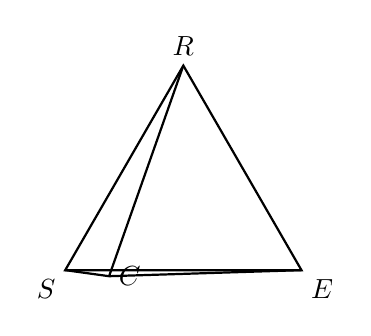
\begin{tikzpicture}[scale=3]

% vertices of a tetrahedron
\coordinate (S) at (0,0,0);
\coordinate (E) at (1,0,0);
\coordinate (R) at (0.5,0.866,0);
\coordinate (C) at (0.5,0.2887,0.8165);

% edges
\draw[thick] (S) -- (E) -- (R) -- cycle;
\draw[thick] (S) -- (C);
\draw[thick] (E) -- (C);
\draw[thick] (R) -- (C);

% labels
\node[below left] at (S) {$S$};
\node[below right] at (E) {$E$};
\node[above] at (R) {$R$};
\node[right] at (C) {$C$};

\end{tikzpicture}
\caption{Regular 3-simplex representing the SERC state space. Each vertex corresponds to dominance of a single component.}
\end{figure}

\newpage

\subsection*{B.2 Zero Point $P_0$ as the Barycentric Center}

\begin{figure}[h!]
\centering
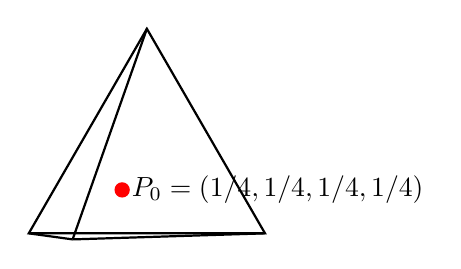
\begin{tikzpicture}[scale=3]

% vertices
\coordinate (S) at (0,0,0);
\coordinate (E) at (1,0,0);
\coordinate (R) at (0.5,0.866,0);
\coordinate (C) at (0.5,0.2887,0.8165);

% edges
\draw[thick] (S) -- (E) -- (R) -- cycle;
\draw[thick] (S) -- (C);
\draw[thick] (E) -- (C);
\draw[thick] (R) -- (C);

% P0 point (barycenter)
\coordinate (P0) at (0.5,0.2887,0.2722);
\filldraw[red] (P0) circle (0.03);

\node[right] at (P0) {$P_0 = (1/4,1/4,1/4,1/4)$};

\end{tikzpicture}
\caption{The Zero Point $P_0$ as the barycentric center of the simplex. It is the unique global minimum of the coherence functional $Q(Z)$.}
\end{figure}

\newpage

\subsection*{B.3 Example Relational Trajectory and Relaxation Toward $P_0$}

\begin{figure}[h!]
\centering
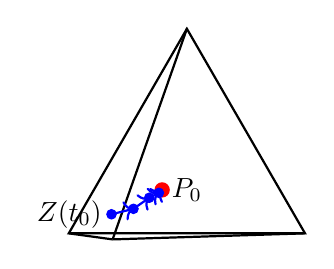
\begin{tikzpicture}[scale=3]

% vertices
\coordinate (S) at (0,0,0);
\coordinate (E) at (1,0,0);
\coordinate (R) at (0.5,0.866,0);
\coordinate (C) at (0.5,0.2887,0.8165);

% edges
\draw[thick] (S) -- (E) -- (R) -- cycle;
\draw[thick] (S) -- (C);
\draw[thick] (E) -- (C);
\draw[thick] (R) -- (C);

% P0
\coordinate (P0) at (0.5,0.2887,0.2722);
\filldraw[red] (P0) circle (0.03);

% trajectory points
\coordinate (Z1) at (0.2,0.1,0.05);
\coordinate (Z2) at (0.32,0.15,0.12);
\coordinate (Z3) at (0.41,0.22,0.18);
\coordinate (Z4) at (0.47,0.26,0.23);

% trajectory lines
\draw[blue, thick, ->] (Z1) -- (Z2);
\draw[blue, thick, ->] (Z2) -- (Z3);
\draw[blue, thick, ->] (Z3) -- (Z4);
\draw[blue, thick, ->] (Z4) -- (P0);

% trajectory points
\filldraw[blue] (Z1) circle (0.02);
\filldraw[blue] (Z2) circle (0.02);
\filldraw[blue] (Z3) circle (0.02);
\filldraw[blue] (Z4) circle (0.02);

\node[right] at (P0) {$P_0$};
\node[left] at (Z1) {$Z(t_0)$};

\end{tikzpicture}
\caption{Example relational trajectory $Z(t)$ approaching the Zero Point $P_0$. The path length corresponds to internal time $T$.}
\end{figure}
\newpage
\begin{thebibliography}{9}
\bibitem{serc2026}
L. Papiernik, \textit{SERC Unified Relational Simplex Metric}, 2026.
\end{thebibliography}

\end{document}
